% !TeX encoding = UTF-8
% !TeX root = choix_extensions.tex
\chapter{Gérer les graphiques}
\label{ch:graphiques}





\section{Texte et figure en parallèle}



\subsection{Figure sans légende - raccourcis}

Le fichier \lstinline!preambule_college.sty! contient des raccourcis basés sur les \lstinline!minipage! : \newline
\lstinline!\txtfig{taille_texte en %}{texte}{figure}! et \lstinline!\figtxt{taille_figure en %}{figure}{texte}! :


%\setlength\fboxsep{0pt}
%\setlength{\txtWidth}{(\linewidth - \widthof{\quad}) * \real{.65}}
%\setlength{\figWidth}{\linewidth - \widthof{\quad} - \txtWidth }
%\noindent
%\begin{minipage}[m]{\txtWidth}
%	{Texte en parallèle d'une figure.}
%\end{minipage}% %N.B. le % est nécessaire pour éviter un espace inter-mot supplémentaire entre les minipages
%\hfill
%\begin{minipage}[m]{\figWidth}
%	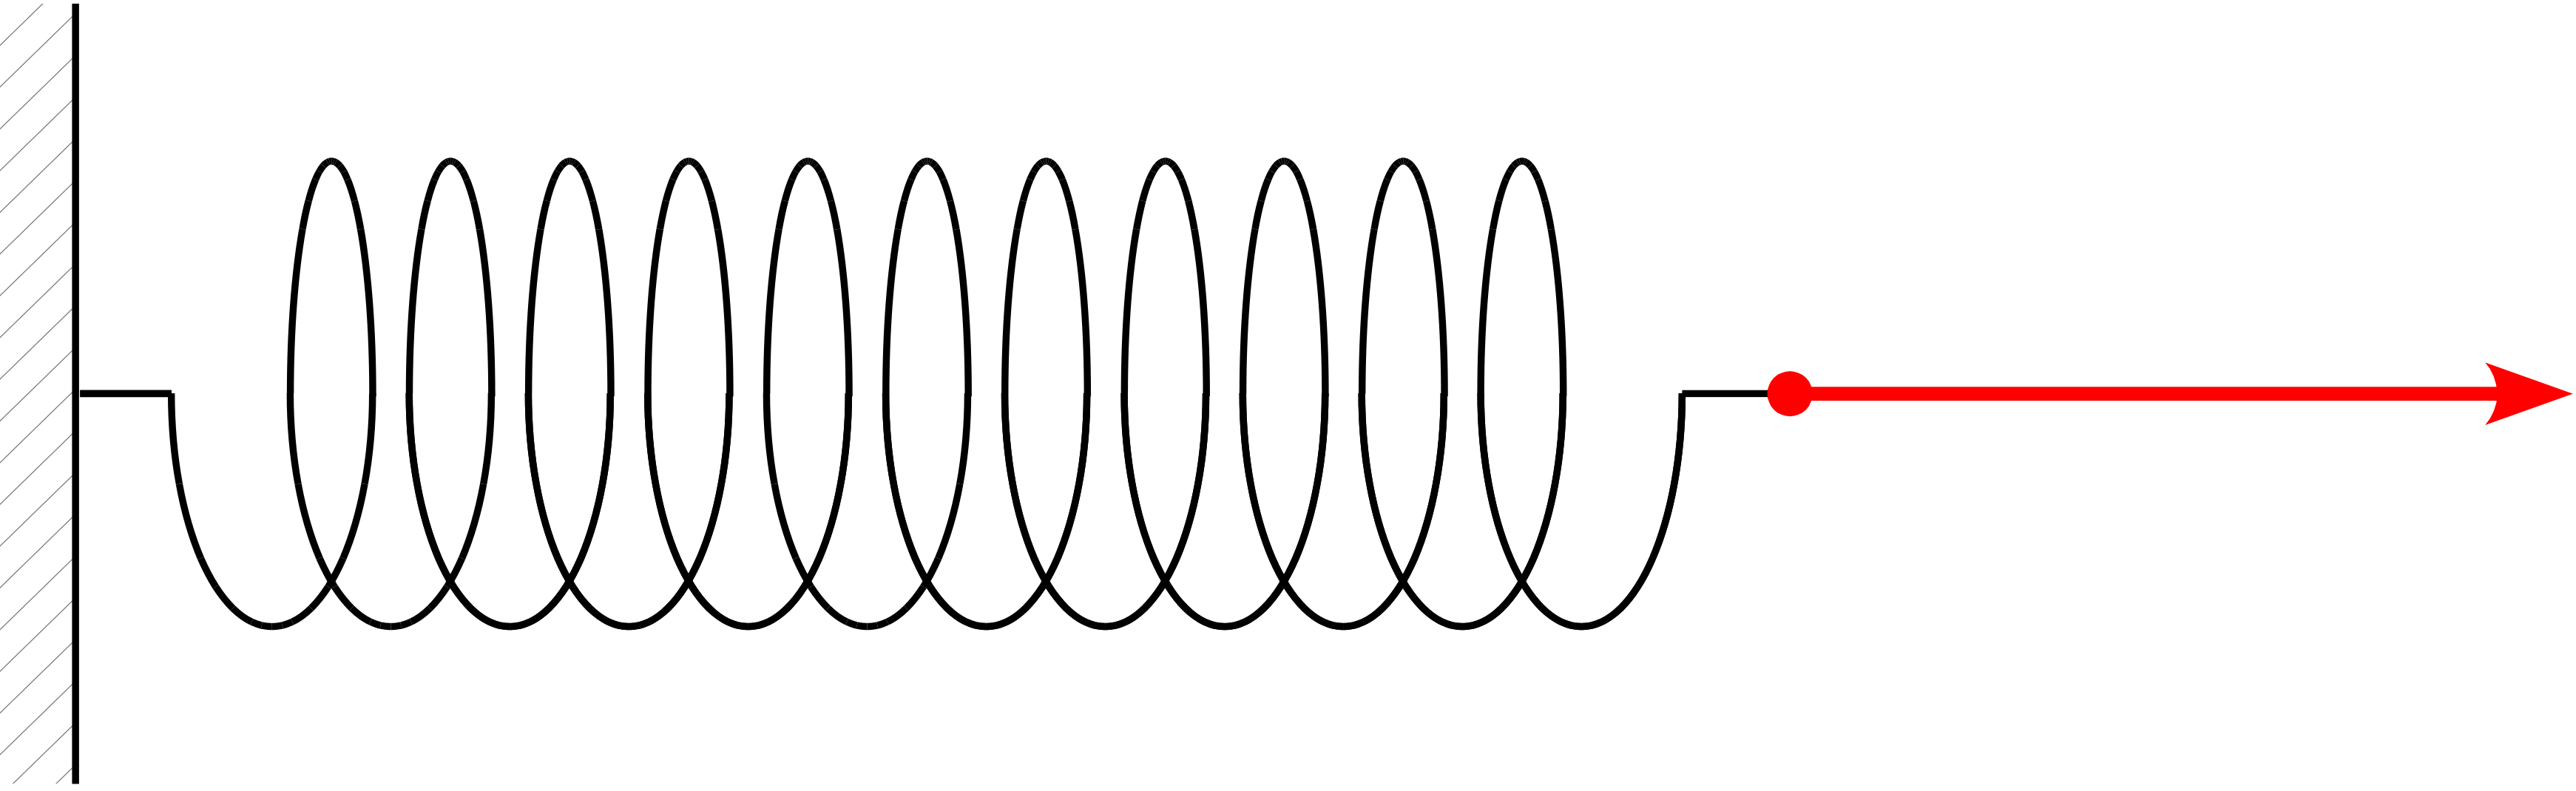
\includegraphics[width=\linewidth]{images/vecteur_force}
%\end{minipage}


\begin{LTXexample}[pos=o]
\txtfig{.65}
  {Texte en parallèle d'une figure.}
  {images/vecteur_force}
\end{LTXexample}

\begin{LTXexample}[pos=o]
\figtxt{.65}
  {images/vecteur_force}
  {Texte en parallèle d'une figure.}
\end{LTXexample}


\subsection{Figure sans légende - à la main}

Presque la même, mais à la main : on peut ainsi jouer sur les paramètres de centrage des minipages. Par exemple, ici avec le paramètre \lstinline![m]! (milieu) :

\begin{LTXexample}[pos=o]
\begin{minipage}[m]{.58\linewidth}
    Texte en parallèle d'une figure.
\end{minipage}% %Un % est nécessaire ici
\hfill
\begin{minipage}[m]{.38\linewidth}
    \centering
%    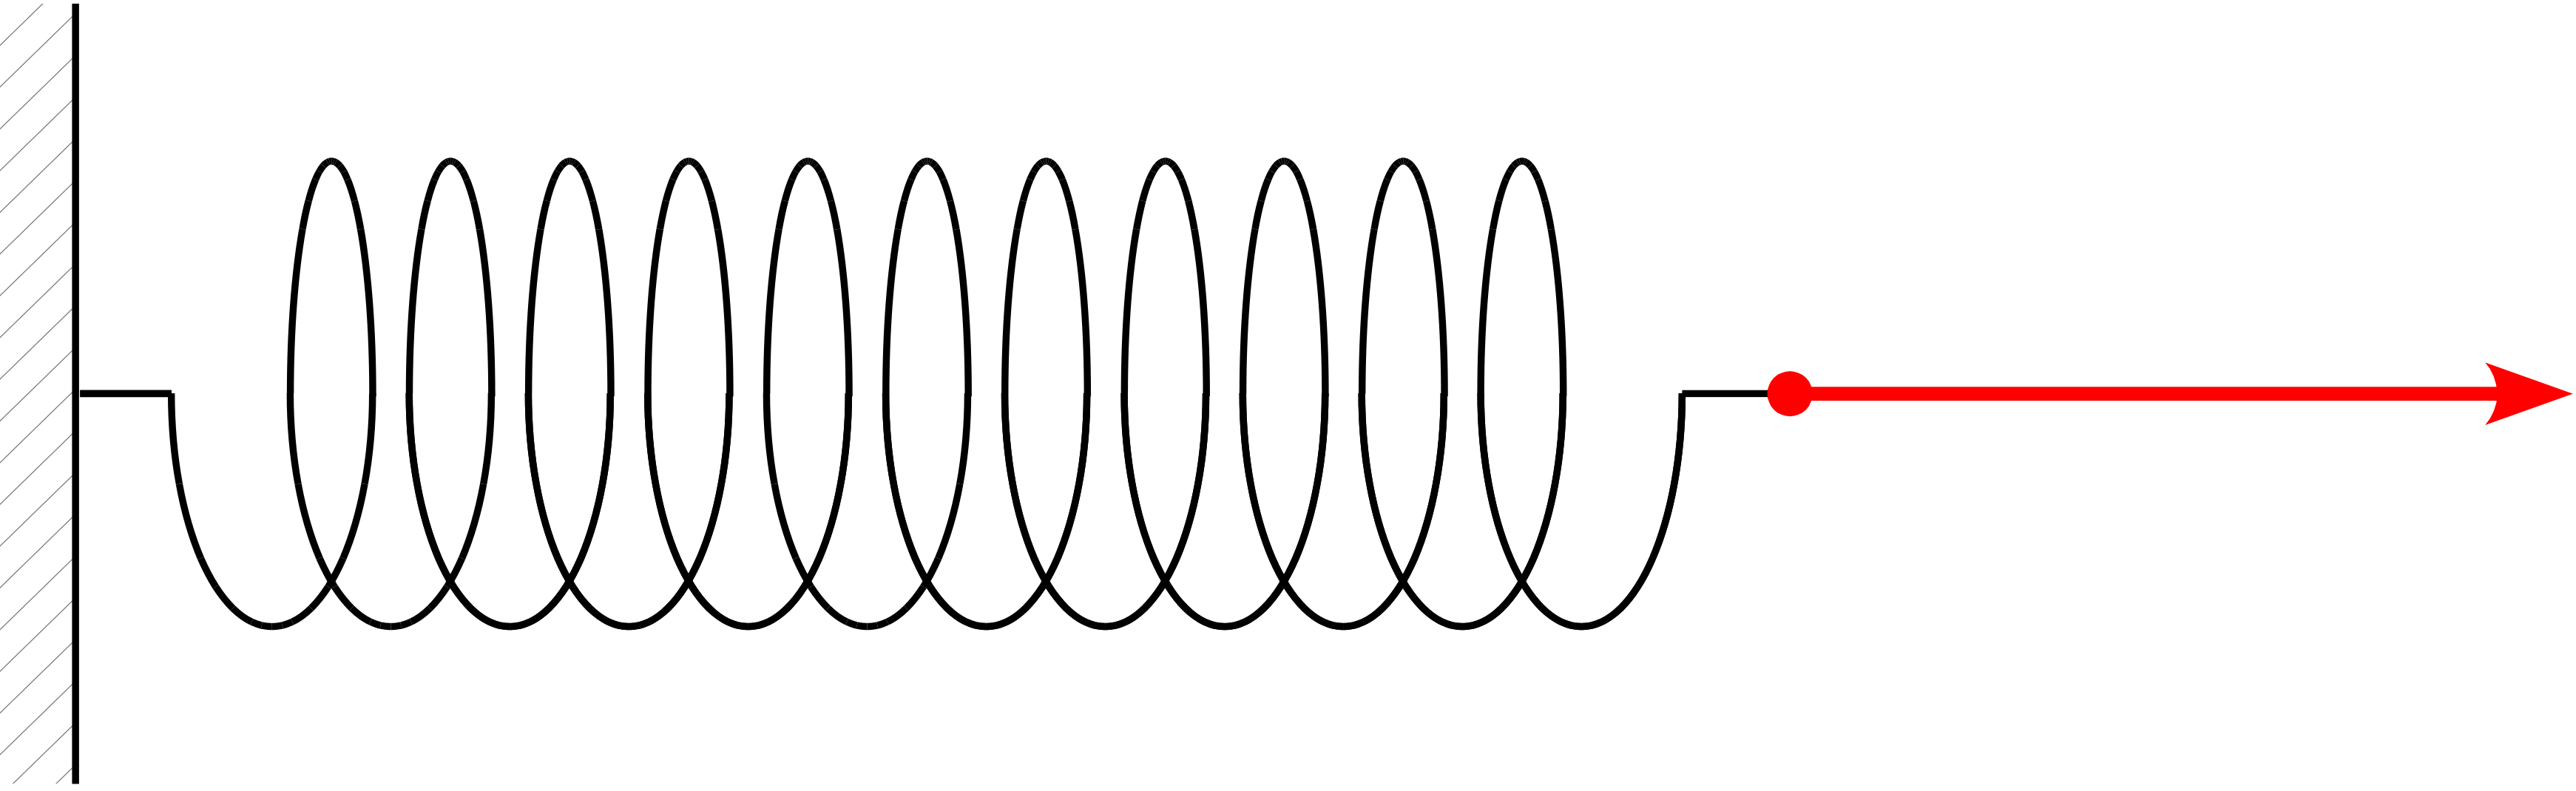
\includegraphics[width=\linewidth]{images/vecteur_force}
\end{minipage}
\end{LTXexample}



\subsection{Figure avec légende}

\begin{LTXexample}[pos=o]
\begin{minipage}[m]{.58\linewidth}
    Texte en parallèle d'une figure.
\end{minipage}% %Un % est nécessaire ici
\hfill
\begin{minipage}[m]{.38\linewidth}
    \centering
%    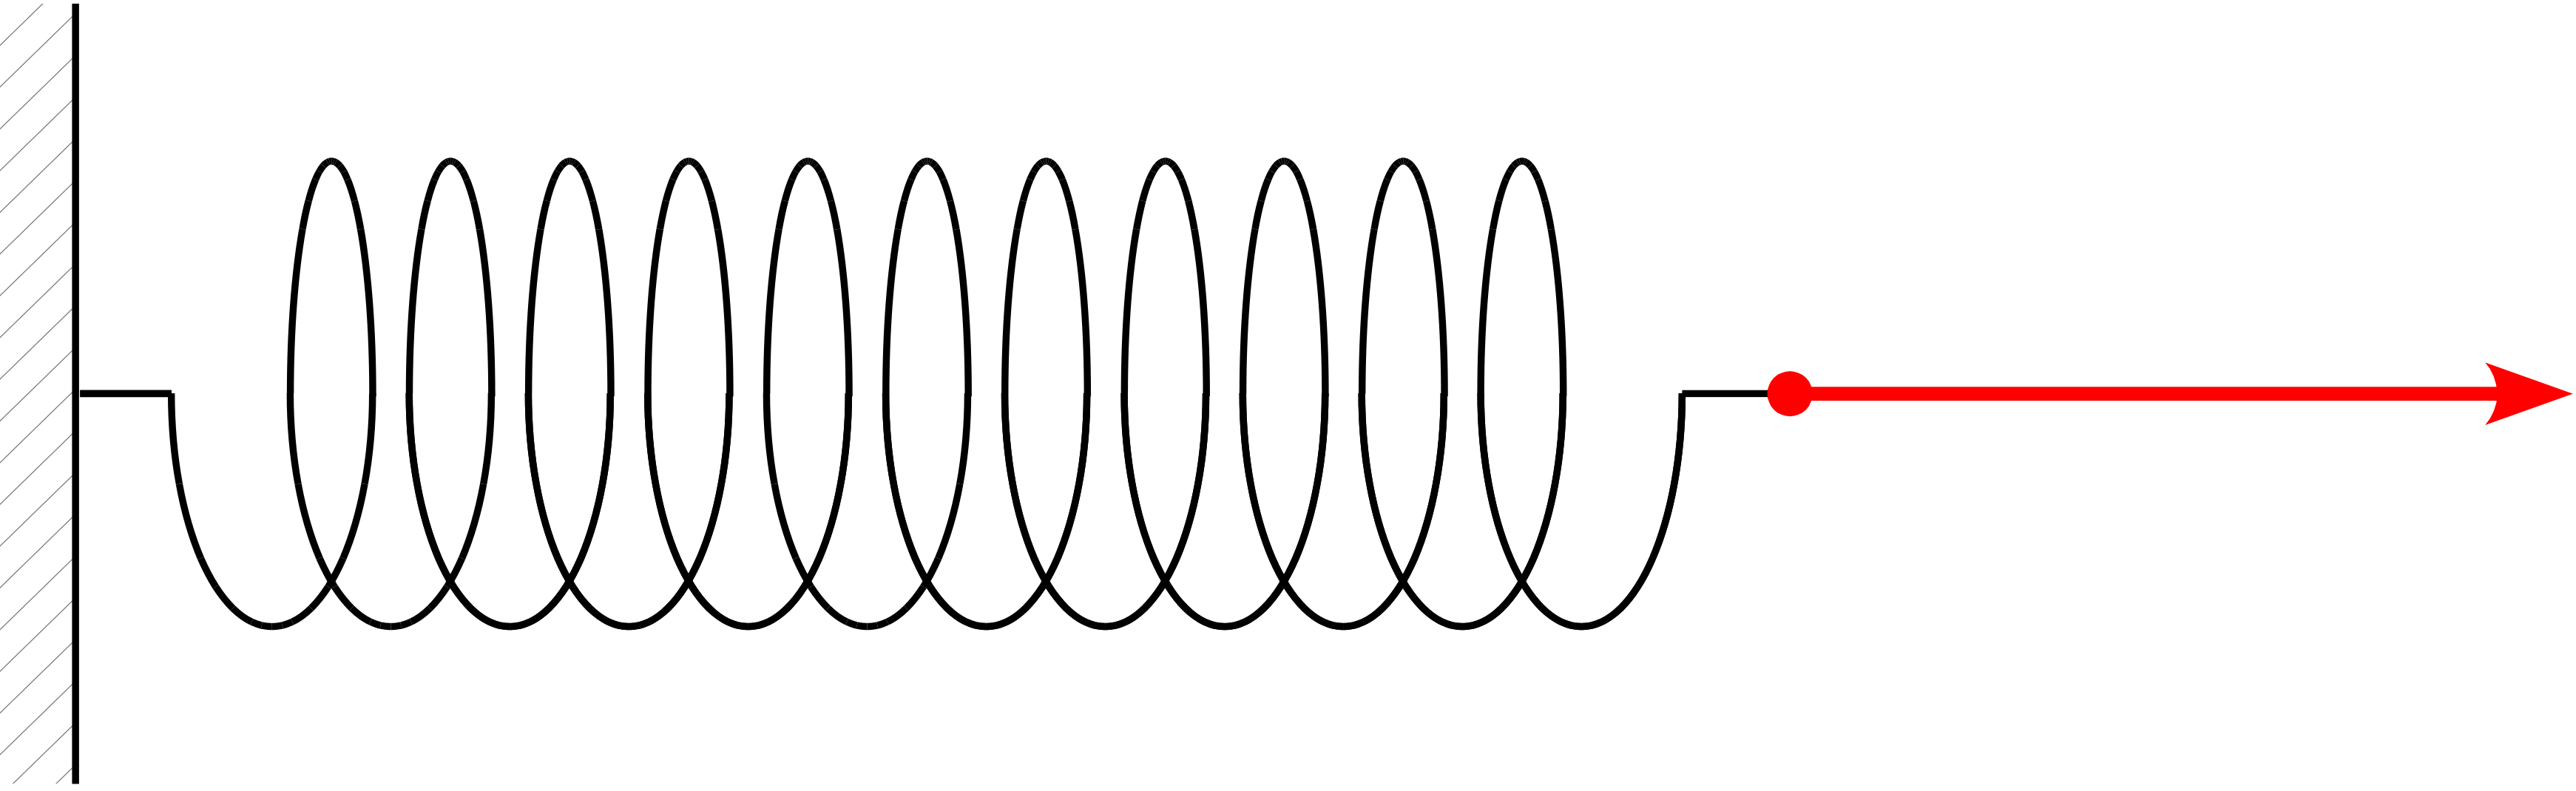
\includegraphics[width=\linewidth]{images/vecteur_force}
    \captionof{figure}{Force}
\end{minipage}
\end{LTXexample}

\remarques*{
	\listtopsep
	\begin{enumerate}
		\item Attention \mintinline{latex}{\captionof{figure}{...}} de l'extension \href{http://www.ctan.org/pkg/caption}{caption} permet d'insérer une légende dans une minipage, mais peut chambouler l'ordre de la numérotation pour les figures à proximité. Il faut vérifier le placement des autres figures autour de celle-ci.
		\item On peut aussi faire ce type de mise en page avec l'extension \mintinline{latex}{float} et \mintinline{latex}{\begin{figure}[H]}, mais ceci n'est pas entièrement compatible avec l'usage de l'extension \mintinline{latex}{minitoc}.
	\end{enumerate}
}





\section{Sous-figures}
\label{sec:textFig}

\begin{minipage}[m]{.48\linewidth}
	\begin{minted}{latex}
\begin{figure}{\linewidth}
  \centering
  \captionsetup{type=figure}
  \subcaptionbox
    {Lentille biconvexe\label{fig:l1}}
    [.45\linewidth]
    {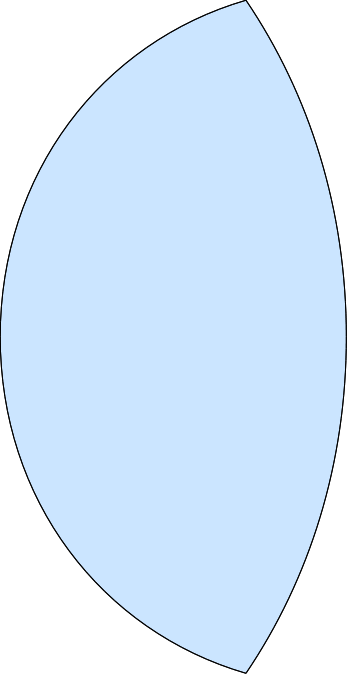
\includegraphics{images/lentille1}
  }
  \quad
  \subcaptionbox
    {Ménisque à bord mince\label{fig:l2}}
    [.45\linewidth]{
    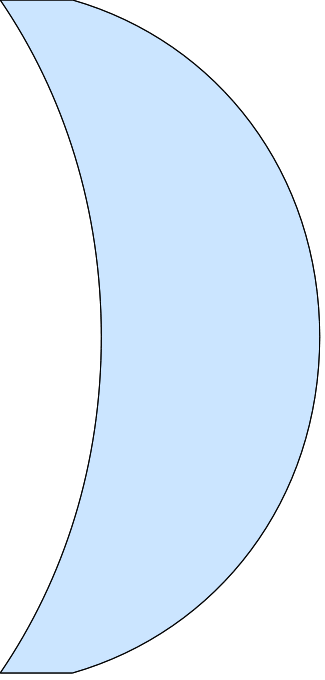
\includegraphics{images/lentille2}
  }
  \caption{Lentilles convergentes
  	\subref{fig:l1} et \subref{fig:l2}}
  \label{fig:lentillesTypes}
\end{figure}
	\end{minted}
\end{minipage}
\hfill
\begin{minipage}[m]{.48\linewidth}
	\begin{figure}[H]%{\linewidth}
		\centering
		\captionsetup{type=figure}
		\subcaptionbox{Lentille biconvexe\label{fig:l1}}[.45\linewidth]{
			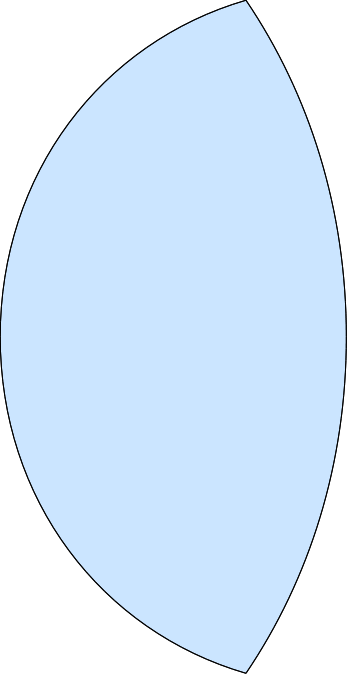
\includegraphics{images/lentille1}
		}
		\quad
		\subcaptionbox{Ménisque à bord mince\label{fig:l2}}[.45\linewidth]{
			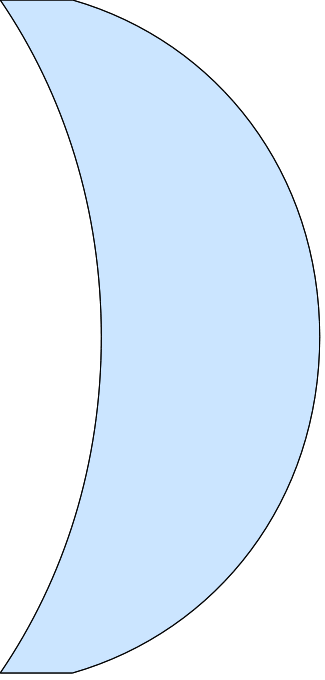
\includegraphics{images/lentille2}
		}
		\caption{Lentilles convergentes
			\subref{fig:l1} et \subref{fig:l2}}
		\label{fig:lentillesTypes}
	\end{figure}
\end{minipage}


\remarque*{
	L'extension \mintinline{latex}{\href{http://mirror.ctan.org/macros/latex/contrib/subfig/subfig.pdf}{subfig}} permet aussi de faire ce type de mise en page, mais elle a des incompatibilités avec \mintinline{latex}{hyperref}.
%	\begin{minipage}[m]{.48\linewidth}
%		\begin{minted}{latex}
%	\begin{figure}[H]
%	  \centering
%	  \subfloat[Lentille biconvexe]{
%	    \includegraphics[width=2.5cm]
%	      {images/lentille1}}
%	    \label{a}
%	   }
%	  \quad
%	  \subfloat[Ménisque à bord mince]{
%	    \includegraphics[width=2.5]
%	      {images/lentille2}
%	     }
%	    \label{b}
%	  }
%	  \caption{Lentilles convergentes}
%	  \label{fig:lentillesTypes}
%	\end{figure}
%		\end{minted}
%	\end{minipage}
%	\hfill
%	\begin{minipage}[m]{.48\linewidth}
%		\begin{figure}[H]
%			\centering
%		  	\subfloat[Lentille biconvexe]{
%		    \makebox[2.5cm]{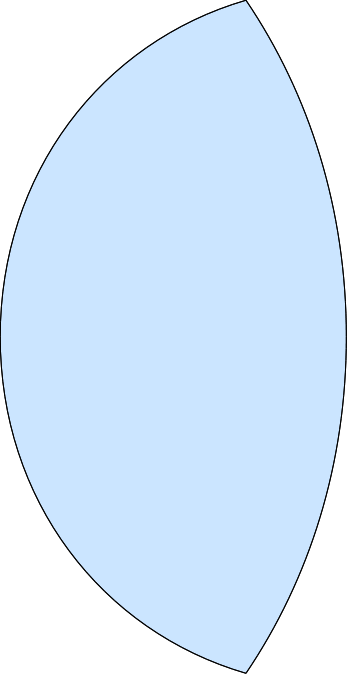
\includegraphics{images/lentille1}}
%		    \label{a}
%		  }
%		  \quad
%		  \subfloat[Ménisque à bord mince]{
%		    \makebox[2.5cm]{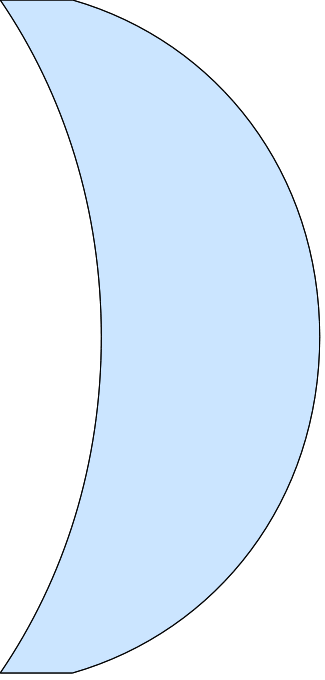
\includegraphics{images/lentille2}}
%		    \label{c}
%		  }
%		  \caption{Lentilles convergentes}
%		  \label{fig:lentillesTypes}
%		\end{figure}
%	\end{minipage}
}





\section{Alignement horizontal des minipages}

Si on veut aligner correctement le haut de deux \mintinline{latex}{minipages} (deux options \mintinline{latex}{[t]}), il se peut que le résultat ne soit pas celui escompté (voir code ci-après) :

\begin{LTXexample}[pos=o,width=.4]
\begin{minipage}[t]{4cm}
  \[
    \cS_{B'CC'} = \cS_{B'BC'}
  \]
\end{minipage}
\hfill
\begin{minipage}[t]{2cm}
  \centering
  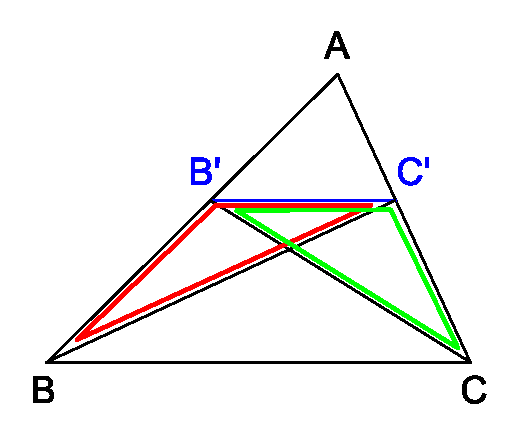
\includegraphics
    [width=.8\linewidth]
    {images/Thales_thm_Thales_dem_01}
\end{minipage}
\end{LTXexample}

Pour éviter cela, il suffit de rajouter \mintinline{latex}{\vspace{0pt}} dans la deuxième \mintinline{latex}{minipage} de manière à donner un point de référence correct à \LaTeX.

\begin{LTXexample}[pos=o,width=.4]
\begin{minipage}[t]{4cm}
  \[
    \cS_{B'CC'} = \cS_{B'BC'}
  \]
\end{minipage}
\hfill
\begin{minipage}[t]{2cm}
  \vspace{0pt}
  \centering
  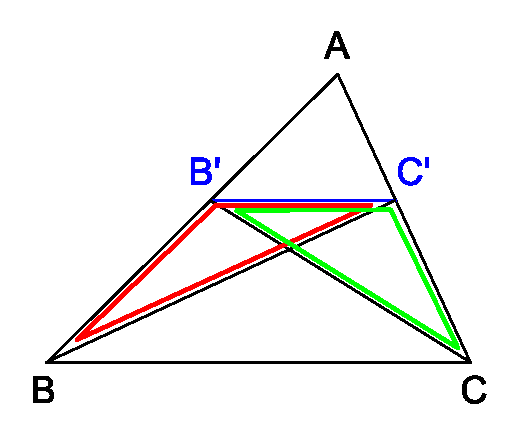
\includegraphics
    [width=.8\linewidth]
    {images/Thales_thm_Thales_dem_01}
\end{minipage}
\end{LTXexample}





\section{Processus d'export des figures GeoGebra}



\subsection{GeoGebra}

GeoGebra est l'outil idéal pour la création de figures géométriques. Il est libre, disponible sur toutes les plates-formes, son développement est très actif et sa communauté d'utilisateur est vaste.

Le \href{http://www.geogebra.org/download}{télécharger} et l'installer (ou non : on peut l'utiliser directement dans son navigateur\dots)




\subsection{Variante choisie : exporter en PGF/TikZ}

Exporter en PGF/TikZ offre le plus grand contrôle sur le résultat final. Pour une variante plus simple, voir \ref{sec:variantesExportGeoGebra}. Ce processus permet de :

\begin{itemize}
	\item présenter des figures sans pixellisation, quel que soit le niveau de zoom voulu;
	\item modifier l'image depuis le document \LaTeX : position des objets, couleurs, épaisseurs des traits, terminaison des flèches\dots
	\item avoir des fontes et des tailles de caractères homogènes entre la figure et le document;	
	\item garantir l'homogénéité des figures dans tout le document et modifier de manière centralisée leur apparence;
	\item pouvoir modifier les images sans créer de catastrophes dans le document final (plus le même niveau de zoom, caractères trop grands ou trop petits\dots);
	\item avoir des fichiers images de faible taille.
\end{itemize}



\subsection{Export de Geogebra}
\label{sec:exportDeGeogebra}

\begin{enumerate}
	\item Pour éviter les problèmes d'échelle et de zoom\footnote{Modifier l'échelle ou le zoom après-coup amène des problèmes de tailles de police de caractères inhomogènes.}, le plus simple est de tracer directement ses figures à la bonne taille ! Pour cela, on peut vérifier la taille voulue dans le document \LaTeX \ (voir \ref{sec:gestionLongueurs}) puis créer un cadre de cette taille dans GeoGebra et faire tenir sa figure dans ce cadre. Dans le document d'exemple, le cadre est défini comme objet auxiliaire de GeoGebra pour le masquer facilement dans la liste des objets.
	\item Ajuster la fenêtre GeoGebra pour que la partie \incmd{Graphique} de GeoGebra corresponde exactement au cadre qui contient la figure.
	\item Masquer le cadre.
	\item Dans TexStudio : menu \incmd{Fichier} \textrightarrow \incmd{Exporter} \textrightarrow \incmd{Graphique vers PGF/TikZ ...}.
	\item Dans la fenêtre d'export, si nécessaire, régler plus finement la zone à exporter, puis \newline \incmd{Générer le code PGF/TikZ}, \incmd{Sauvegarde...}  et \incmd{sauvegarder}. Ceci crée un fichier \incmd{.tex}
\end{enumerate}



\subsection{Réglages dans le fichier \mintinline{bash}{.tex}}

\remarque*{
	Pour donner à toutes les figures la même ligne graphique, il faut définir au préalable des styles \incmd{TikZ} de manière centralisée. Le fichier \incmd{preambule_personnalisation.sty} en comprend déjà une série sous forme de commandes \mintinline{latex}{\tikzset{}}.
}

Il est plus facile et plus rapide, notamment à la compilation, de faire les réglages dans ce document intermédiaire que dans le document final.

\begin{itemize}
	\item Les étiquettes des objets : supprimer \mintinline{latex}{\begin{scriptsize}} et \mintinline{latex}{\end{scriptsize}}, régler les positions, changer les caractères spéciaux\dots
	\item Copier-coller les styles prédéfinis (les \incmd{tikzset{}}) dans le préambule pour qu'ils soient disponibles à la compilation.
	\item Remplacer les styles graphiques (couleurs, épaisseurs de traits\dots) par ses propres styles.
\end{itemize}

Lorsque la figure est au point, on copie tout l'environnement \incmd{tikzpicture} et on le colle dans un fichier \incmd{.tikz}.



\subsection{Import dans le document \LaTeX}


Le fichier \incmd{preambule_college.sty} appelle l'extension \incmd{tikzscale} qui permet d'appeler le fichier \incmd{.tikz} comme n'importe quel fichier image : \mintinline{latex}{\includegraphics{figures/fichier.tikz}}. Cela permet aussi d'utiliser, avec modération, les options habituelles, notamment \mintinline{latex}{width}, \mintinline{latex}{height}, \mintinline{latex}{scale}\dots.


\begin{minipage}[m]{.48\linewidth}
	\begin{minted}{latex}
\begin{figure}[H]
  \centering
  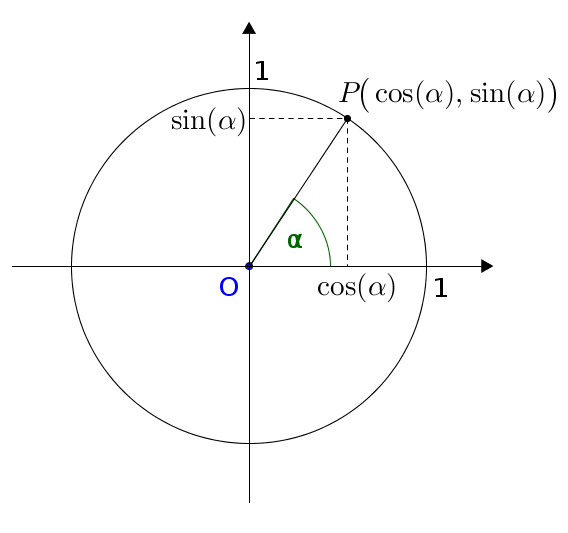
\includegraphics[width=\linewidth]
    {figures/fig_11_05_cercle_cos_sin.tikz}
  \label{fig:11_05_cercle_cos_sin}
  \vspace*{-5ex}
  \caption{}
\end{figure}
	\end{minted}
\end{minipage}
\hfill
\begin{minipage}[m]{.48\linewidth}
	\begin{figure}[H]
		\centering
		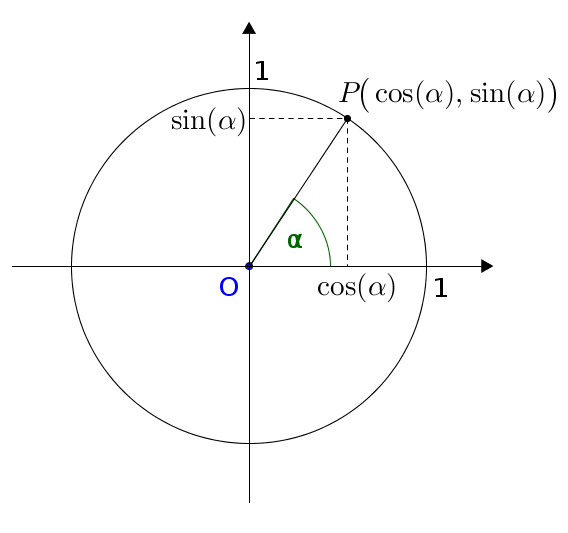
\includegraphics[width=\linewidth]{figures/fig_11_05_cercle_cos_sin.tikz}
		\label{fig:11_05_cercle_cos_sin}
		\vspace*{-5ex}
		\caption{}
	\end{figure}
\end{minipage}



\subsection{Variantes}
\label{sec:variantesExportGeoGebra}

Le processus ci-dessus est la plus propre et la plus souple, mais un peu compliqué. Dans tous les cas, ça vaut la peine de suivre les trois premiers points de \ref{sec:exportDeGeogebra}. Puis, on peut choisir une des variantes suivantes :
\begin{enumerate}
	\item Variante "quick \& dirty" : exporter au format \incmd{.png}. C'est un bitmap, donc il pixelise si on l'agrandit, la police de caractère n'est pas la même, il n'y a aucun moyen de faire des retouches. Réglage à vérifier : police de caractère de GeoGebra en \SI{24}{pt} et échelle eps \incmd{1:1}.
	\item Variante "quick \& juste un peu moins dirty" : exporter au format \incmd{eps} ou \incmd{pdf}. L'export se fait en format vectoriel. La définition est donc parfaite, mais il n'y a toujours pas de possibilité de retouche. Privilégier le \incmd{.eps} puisque le compilateur PDFLaTeX de \TeX \ Live sait gérer les deux formats\footnote{Il crée silencieusement un fichier \incmd{.pdf} qu'il appelle ensuite.}.\\
	\begin{minipage}{.48\linewidth}
		\begin{figure}[H]
			\centering
			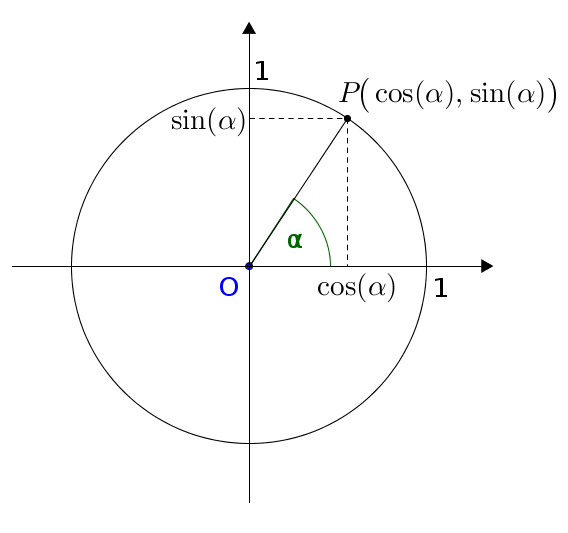
\includegraphics[width=\linewidth]{figures/fig_11_05_cercle_cos_sin.png}
			\label{fig:11_05_cercle_cos_sin2}
			\vspace*{-5ex}
			\caption{Export en png}
		\end{figure}
	\end{minipage}
	\hfill
	\begin{minipage}{.48\linewidth}
		\begin{figure}[H]
			\centering
			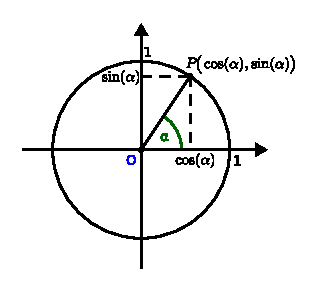
\includegraphics[width=\linewidth]{figures/fig_11_05_cercle_cos_sin.eps}
			\label{fig:11_05_cercle_cos_sin2}
			\vspace*{-5ex}
			\caption{Export en eps}
		\end{figure}
	\end{minipage}
\end{enumerate}

\remarque*{
	Avec ces variantes, il est possible de définir la zone d'export précisément. On peut définir deux points appelés $\text{Export}_1$ (en haut à gauche) et $\text{Export}_2$ (en bas à droite). Si ces deux points sont dans la zone affichée à l'écran, seul le rectangle défini par ces deux points sera exporté.
}
